\documentclass[]{aiaa-tc} % insert '[draft]' option to show overfull boxes
\renewcommand{\thesection}{\Roman{section}}
\renewcommand{\thesubsection}{\Alph{subsection}}
%---------- USER-ADDED PACKAGES
\usepackage{abstract}
\usepackage{amsmath}
\usepackage[english]{babel}
\usepackage{booktabs} 	% For tables
\usepackage{breqn}
\usepackage{caption} 	% For subfigures
\usepackage[capitalise]{cleveref}
\usepackage{float}
\usepackage[T1]{fontenc}
\usepackage{gensymb}
\usepackage{geometry}
\usepackage{graphicx}
\usepackage{import}		% Package for breaking down lengthy documents into submodules
\usepackage[utf8x]{inputenc}
\usepackage{lettrine}
\geometry{legalpaper, margin=1in}
\usepackage{pdfpages} 	% To include PDF pages in appendix
\usepackage{placeins}	% Floatbarrier
\usepackage{siunitx} 	% For the degree symbol "\ang{}"
\usepackage{subcaption} % For subfigures
\usepackage{wrapfig}	% For inline figures
\usepackage{type1cm}
\usepackage{listings} %--- For including MATLAB code ---%
\usepackage{color} %red, green, blue, yellow, cyan, magenta, black, white
\definecolor{mygreen}{RGB}{28,172,0} % color values Red, Green, Blue
\definecolor{mylilas}{RGB}{170,55,241}
\lstset{language=Matlab,%
	basicstyle=\footnotesize\ttfamily,
	breaklines=true,%
	morekeywords={matlab2tikz},
	keywordstyle=\color{blue},%
	morekeywords=[2]{1}, keywordstyle=[2]{\color{black}},
	identifierstyle=\color{black},%
	stringstyle=\color{mylilas},
	commentstyle=\color{mygreen},%
	showstringspaces=false,%without this there will be a symbol in the places where there is a space
	numbers=left,%
	numberstyle={\tiny \color{black}},% size of the numbers
	numbersep=9pt, % this defines how far the numbers are from the text
	emph=[1]{for,end,break},emphstyle=[1]\color{red}, %some words to emphasise
	%emph=[2]{word1,word2}, emphstyle=[2]{style},    
}
%---End MATLAB code inclusion package ---%

% ---------------------------------
% Variables
\newcommand{\figwidth}{3.4in}				% Width of single figure
\newcommand{\figheight}{2.43in}				% Height of single figure
\newcommand{\figwidthlegend}{4.0in}			% Width of single figure with outer legend
\newcommand{\doubfigf}{.475}				% Text width factor in double figure
\AtBeginDocument{\renewcommand{\abstractname}{}}

% Data used by 'handcarry' option if invoked
\AIAApapernumber{2019}
\AIAAconference{SciTech, January 2019, San Diego CA}
\AIAAcopyright{\AIAAcopyrightD{2019}}

%%%%%%%%%%%%%%%%%%%%%%%%%%%%%%%%%%%%%%%%%%%%%%%%%%%%%%%%%%%%%%%%%
% COVER PAGE
%%%%%%%%%%%%%%%%%%%%%%%%%%%%%%%%%%%%%%%%%%%%%%%%%%%%%%%%%%%%%%%%%
\title{Best Practices for Wake Model and Optimization Algorithm Selection in Wind Farm Layout Optimization.}

\author{Nicholas F. Baker\thanks{Masters Student, Brigham Young University Department of Mechanical Engineering},\  Andrew P. J. Stanley\thanks{Ph.D. Candidate, Brigham Young University Department of Mechanical Engineering}, \ Jared Thomas\thanks{Ph.D. Student, Brigham Young University Department of Mechanical Engineering}, \ and Andrew Ning\thanks{Assistant Professor, Brigham Young University Department of Mechanical Engineering} \\
	{\normalsize\itshape Brigham Young University, Provo, Utah 84602.}\\
Katherine Dykes\thanks{Senior Engineer, National Wind Technology Center}\\
	\normalsize\itshape National Renewable Energy Laboratory, Golden, Colorado 80401}

\begin{document}
\maketitle{}

\import{./sections/}{iea37-wflocs-abst.tex}

%\listoftodos

%\section*{Nomenclature}

	%\begin{tabbing}
	%  XXX \= \kill% this line sets tab stop
	%  $J$ \> Jacobian Matrix \\
	%  $f$ \> Residual value vector \\
	%  $x$ \> Variable value vector \\
	%  $F$ \> Force, N \\
	%  $m$ \> Mass, kg \\
	%  $\Delta x$ \> Variable displacement vector \\
	%  $\alpha$ \> Acceleration, m/s\textsuperscript{2} \\[5pt]
	%  \textit{Subscript}\\
	%  $i$ \> Variable number \\
	% \end{tabbing}
	
%%%%%%%%%%%%%%%%%%%%%%%%%%%%%%%%%%%%%%%%%%%%%%%%%%%%%%%%%%%%%%%%%
% INTRODUCTION
%%%%%%%%%%%%%%%%%%%%%%%%%%%%%%%%%%%%%%%%%%%%%%%%%%%%%%%%%%%%%%%%%
\section{Introduction}

	\import{./sections/}{iea37-wflocs-intro.tex}

%%%%%%%%%%%%%%%%%%%%%%%%%%%%%%%%%%%%%%%%%%%%%%%%%%%%%%%%%%%%%%%%%
% METHODOLOGY
%%%%%%%%%%%%%%%%%%%%%%%%%%%%%%%%%%%%%%%%%%%%%%%%%%%%%%%%%%%%%%%%%
\section{Methodology} \label{sec:meth}

	\import{./sections/}{iea37-wflocs-mthd.tex}

%%%%%%%%%%%%%%%%%%%%%%%%%%%%%%%%%%%%%%%%%%%%%%%%%%%%%%%%%%%%%%%%%
% RESULTS
%%%%%%%%%%%%%%%%%%%%%%%%%%%%%%%%%%%%%%%%%%%%%%%%%%%%%%%%%%%%%%%%%
\section{Results} \label{sec:res}

	\import{./sections/}{iea37-wflocs-rslts.tex}

%%%%%%%%%%%%%%%%%%%%%%%%%%%%%%%%%%%%%%%%%%%%%%%%%%%%%%%%%%%%%%%%%
% RESULTS
%%%%%%%%%%%%%%%%%%%%%%%%%%%%%%%%%%%%%%%%%%%%%%%%%%%%%%%%%%%%%%%%%
\section{Conclusion}

%	\import{./sections/}{iea37-wflocs-conc.tex}

%%%%%%%%%%%%%%%%%%%%%%%%%%%%%%%%%%%%%%%%%%%%%%%%%%%%%%%%%%%%%%%%%%%%%%%%%
%							APPENDIX
%%%%%%%%%%%%%%%%%%%%%%%%%%%%%%%%%%%%%%%%%%%%%%%%%%%%%%%%%%%%%%%%%%%%%%%%%
\pagebreak
\section*{Appendix}

\section*{Acknowledgments}
This work is funded by Brigham Young University.

%\newpage
\section{Announcement Document}
\label{app:anndoc}
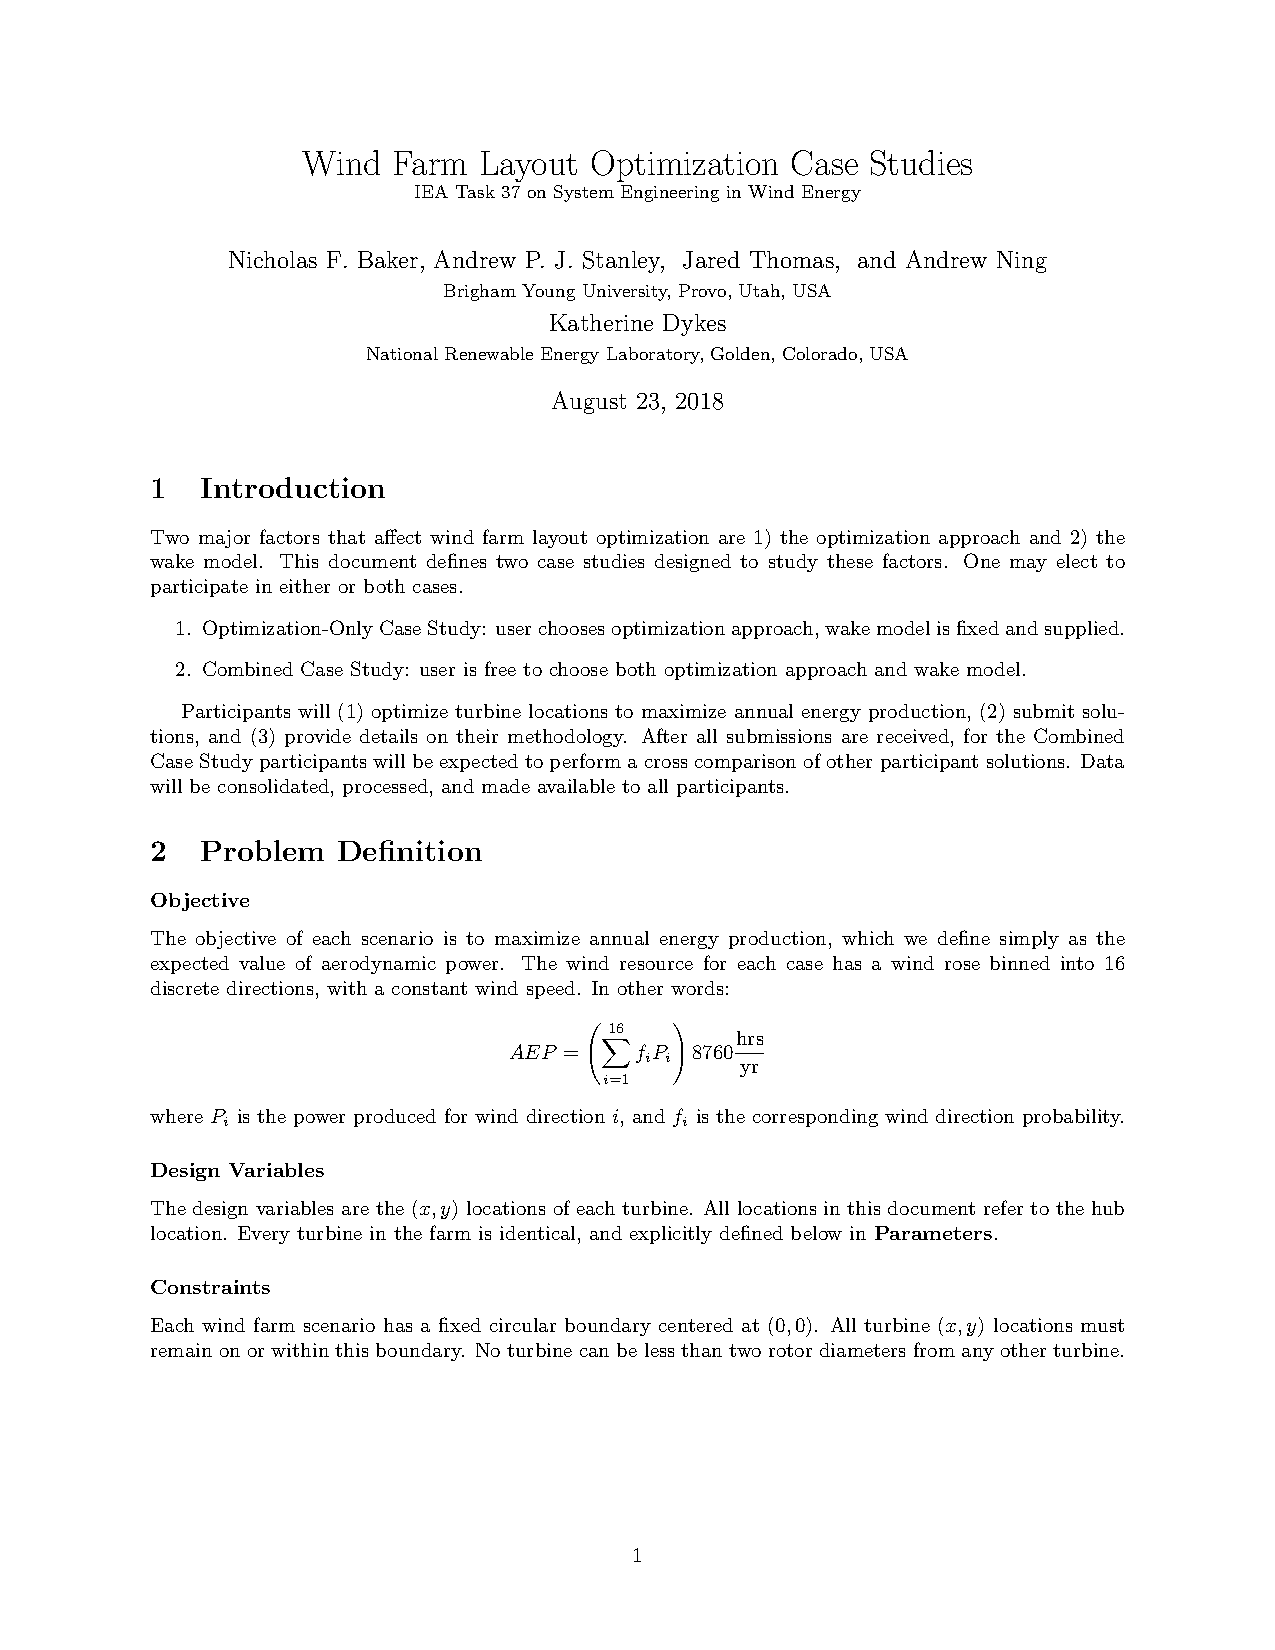
\includepdf[pages={-}]{iea37-wflocs-announcement.pdf}

\section{Python Code}
\label{app:aepcalc}
\lstinputlisting[language=python]{iea37-aepcalc.py}

\FloatBarrier

\pagebreak
\bibliographystyle{aiaa}
\bibliography{aiaa-conf}
\end{document}